\documentclass[11pt,a4paper,twoside]{article}
%%%%%%%%%%%%%%
\usepackage{etoolbox}  % used in jmpag.sty
\usepackage{forloop}    % used in jmpag.sty
%%%%%%%%%%%%%%
\usepackage{amsthm,amsfonts,amsmath,amscd,amssymb}
\usepackage{latexsym}
\usepackage{euscript}
\usepackage{enumitem}
%\usepackage{rotating}
\usepackage{graphicx}
%\usepackage{epstopdf}
\usepackage{tikz}
\usepackage{caption}
\usepackage{subcaption}
\usepackage{cite}
\usepackage[utf8]{inputenc}
\usepackage[english]{babel}
\usepackage{xcolor}
\definecolor{darkgreen}{HTML}{00A000}
\definecolor{darkblue}{HTML}{0000A0}
\definecolor{darkred}{HTML}{D00000}
\usepackage[colorlinks=true]{hyperref}%%%%%%%%%[,backref]!!!!!!!!!!!!!!!!!!!!
\hypersetup{linkcolor=darkred, urlcolor=darkblue, citecolor=darkgreen}%%%%%%%%
%
%%%%%%%%%%%%%%%%%%%%%% YOUR PACKAGES %%%%%%%%%%%%%%%%%%%%%%%%%%%%%%


%%%%%%%%%%%%%%%%%%%%%% END YOUR PACKAGES %%%%%%%%%%%%%%%%%%%%%%%%%%

\usepackage{jmpag}

%%%%%%%%%%%%%%%%%%%%%%%%%%%%%%%%%%%%%%%%%%%%%%%%%%
\tolerance=9000
\textwidth=135mm%11pt
\textheight=216.5mm %196.5mm%11pt
\oddsidemargin=0mm
\evensidemargin=25mm
\topmargin-10mm

\pagestyle{jmpag}

%%%%%%%%%%%%%%%%%%%%%%%%%%%%%%%%%%%%%%%%%%%%%%%%%%%%%%%%%%%%%%

%%%%%%%%%%%%%%%%%%%%%%%%%%%%%%%%%%%%%%%%%%%%%%%%%%%%%%%%%%%%%%%%

\begin{document}

%%%%%%%%%%%%%% TITLE and AUTHORS %%%%%%%%%%%%%%%%%%

% The full title of your paper
\title{Numerical Study of Soliton Solutions to the Two Dimensional Boussinesq  Equation}

% If the title of your paper is too long, use the short title please. It should not exceed 60 symbols (including blank spaces).

%\title[Short Title]{Title}


% Author1
%FirstName1 LastName1
\author{Krassimir Angelow}
%Institution1, address1, City1, Postal Code1, Country
\address{Bulgarian Academy of Sciences, Institute of Mathematics and Informatics, ul. Acad. G. Bonchev, block 8, 1113 Sofia, Bulgaria}
%e-mail1
\email{angelow@math.bas.bg}

% Author2
%FirstName2 LastName2
\author{Natalia Kolkovska}
%Institution2, address2, City2, Postal Code2, Country2
\address{Bulgarian Academy of Sciences, Institute of Mathematics and Informatics, ul. Acad. G. Bonchev, block 8, 1113 Sofia, Bulgaria}
%e-mail2
\email{n.kolkovska@gmail.com}


%%%%%%%%%%%%%%%% END TITLE and AUTHORS %%%%%%%%%%%%%%%%%%%

\BeginPaper %%%%%%% do not remove this command

%%%%%%%%%%%%%%%%%%%%%% MY MACROS %%%%%%%%%%%%%%%%%%%%

\newcommand{\ep}{\varepsilon}
\newcommand{\eps}[1]{{#1}_{\varepsilon}}
\newcommand{\rf}[1]{(\ref{#1})}
\newcommand{\RR}{\mathbb{R}}

%%%%%%%%%%%%%%%%%%%%% END MY MACROS %%%%%%%%%%%%%%%%%%%%%%

%%%%%%%%%%%%%%%%%%%%%%% ABSTRACT %%%%%%%%%%%%%%%%%%%%%%%%

\begin{abstract}
The aim of this paper is to evaluate propagating wave solutions to the two dimensional Boussinesq Equation (BE). To solve this nonlinear fourth order hyperbolic problem we use Fast Poisson Solver with high order finite difference schemes for the spatial derivatives. Taylor Series (TS) expansion about time is used to move the soliton forward. A Boundary Condition (BC) is applied on the computational boundary. Results from the TS approach are compared with results from another known method in the literature. The performed numerical tests exhibit good convergence and confirm the validity of the TS method.



\key{differential equation, two dimensional Boussinesq equation, traveling wave solutions (TWS), high order finite difference schemes, Fast Poisson Solvers.}

\msc{34L15, 34L20, 35R10}
\end{abstract}


%%%%%%%%%%%%%%%%%%%% END ABSTRACT %%%%%%%%%%%%%%%%%%%%%%%%%%%%%

%The title of your section
\section{Introduction.}\label{introduction}

In this paper we  consider the two dimensional Boussinesq  Equation (BE)
\begin{align} \label{eq1}
&u_{tt} - \Delta u -\beta_1  \Delta u_{tt} +\beta_2 \Delta ^2 u + \Delta f(u)=0   \quad \text{for}  (x,y) \in \RR^2, \, t\in\RR^+, 
\\ \nonumber &u(x,y,0)=u_0(x,y), \, u_t(x,y,0)=u_1(x,y)   \quad\text{for} \, (x,y) \in \RR^2,
\\  &u(x,y) \rightarrow 0,  \Delta u(x,y) \rightarrow 0 ,  \quad \text{for}  \sqrt{x^2 + y^2} \rightarrow \infty, \label{eq11}
\end{align}
where   $f(u)=\alpha u^2$,  $\alpha>0$, $\beta_1>0$, $\beta_2>0$  are dispersion parameters, and $\Delta$ is the Laplace operator. The BE is famous with the approximation of shallow water waves or also weakly non--linear long waves. It is often used for simulation of various physical processes e.g. turbulence in fluid mechanics, vibrations in acoustics etc. A derivation of the BE from the original Boussinesq system can be found in \cite{ChChr}.

In previous work \cite{EllipticProblem} and \cite{BoundaryProblem} the stationary BE is studied once again. The obtained results there could serve as initial and boundary condition for the hyperbolic equation \rf{eq1}, \rf{eq11}  here. In order to relate to \cite{EllipticProblem} and \cite{BoundaryProblem}
the following variable change is applied
\begin{equation}\label{vc}
x = \sqrt{\beta_1} \tilde x, \quad y = \sqrt{\beta_1} \tilde y, \quad t = \sqrt{\beta_1} \tilde t, \quad \tilde \Delta = \tilde u_{\tilde x \tilde x} + \tilde u_{\tilde y \tilde y}
\end{equation}
which transforms the main equation \rf{eq1}  into 
\begin{equation}\label{eqVC}
(E-\tilde \Delta)  \tilde u_{\tilde t \tilde t} = \frac{(E-\tilde\Delta)\tilde\Delta \tilde u + \alpha \beta \tilde\Delta(\tilde u^2) + (\beta -1)\tilde\Delta \tilde u}{\beta},
\end{equation}
where $\beta = \beta_1 / \beta_2$. The goal of the article is to seek for soliton solutions to \rf{eqVC}, which 
are traveling  in $y$ direction with velocity $c$. TS expansion is used to calculate the next time layer with respect to the time step $\tau$. The time derivatives
are obtained from the equation \rf{eqVC} by an iterative procedure. This is possible because the equation allows to isolate the highest time derivative on one side of the equation. By differentiating with respect to time variable one could obtain higher time derivative terms in the TS expansion. Here, the solver could be adjusted to use second, fourth or sixth approximation order, i.e. $O(\tau^2)$, $O(\tau^4)$, $O(\tau^6)$. To increase the precision of the numerical method, finite difference schemes (FDS) with local approximation of forth $O(h^4)$ and sixth $O(h^6)$ order are applied to the spatial derivatives i.e.  second derivatives along space are approximated with high order finite differences. Thus, the numerical solution is computed on relatively coarse grid with high accuracy. In order to compare the results from TS method, a conservative finite difference scheme with weights is used, which applies second order of approximation along time and space.
Both methods are tested with zero boundary and also with BC found and developed in \cite{BoundaryProblem}.

%The title of your subsection in the section
\section{Fast Poisson Solvers and Invertion of $(E-\tilde \Delta)$ in \rf{eqVC}}

\begin{lemma} \label{eigenLema} Let the set of all eigenvectors $W :=$ $W_1, W_2, ..., W_n$ of a real matrix $A \in \RR^{n \times n}$ builds an orthogonal basis in $\RR^n$. Let the eigenvalues of $A$ are \{ $\lambda_1, ..., \lambda_n$ \} and further let $AW_i = \lambda_i W_i$ for $i=1,...n$. Then the matrix $\beta E + A$ has the same set of eigenvectors W as A and furthermore $( \beta E + A) W_i = (\beta + \lambda_i)W_i$.
\end{lemma}

\begin{proof}
$(\beta E + A)W_i = \beta W_i + AW_i = \beta W_i + \lambda_i W_i = (\beta + \lambda_i)W_i$.
\end{proof}
Suppose the following linear equaion
\begin{equation}\label{FPeq}
Au:=u-\Delta u = f
\end{equation}
defined on $\Gamma = \{ (0,1) \times (0,1) \}$ with homogeneous Dirichlet boundary conditions $u(x,y) = 0$, $(x,y) \in \partial \Gamma$. The discrete version of \rf{FPeq} - $A_h u_h = f_h$ - using the notations defined in previous sections, is a system of linear equations where $A_h \in \RR^{n^2 \times n^2}$, $f_h, u_h \in \RR^{n^2}$ and n is defined by the relation $h=1/n$. For simplicity the same discretization step $h$ is applied along both space directions. Therefore,
%\begin{equation}\label{MATeq}
\[
A_h = \frac{1}{h^2}
\begin{bmatrix}
    A_{11}       & -E          &  0              & \dots & 0 \\
    -E               & A_{22}  & -E              & \dots & \dots  \\
      \dots         & \searrow     & \searrow  & \searrow  & \dots  \\
      \dots         & \dots     & \dots         & \dots   &    \dots  \\
      \dots         & \dots    & \dots         & \dots & -E  \\
     0                 & \dots   &  0               & -E    & A_{nn}
\end{bmatrix}
,
u_h = 
\begin{bmatrix}
    \bar u_{1} \\
    \bar u_{2}  \\
    \vdots  \\
    \vdots  \\
    \bar u_{n}
\end{bmatrix}
,
f_h = 
\begin{bmatrix}
    \bar f_{1} \\
    \bar f_{2}  \\
    \vdots  \\
    \vdots  \\
    \bar f_{n}
\end{bmatrix}
\]
where $\bar u_k = (u_{k,1}, u_{k,2}, ..., u_{k,n})\in \RR^{n}$ and $\bar f_k = (f_{k,1}, f_{k,2}, ..., f_{k,n})\in \RR^{n}$. Furthermore, $A_{i,i} \in \RR^{n \times n}$, $i = 1, ..., n$ is defined as
\[
A_{i,i} = 
\begin{bmatrix}
    4+h^2       & -1          &  0              & \dots & 0 \\
    -1               & 4+h^2  & -1              & \dots & \dots  \\
      \dots         & \searrow     & \searrow  & \searrow  & \dots  \\
      \dots         & \dots     & \dots         & \dots   &    \dots  \\
      \dots         & \dots    & \dots         & \dots & -1  \\
     0                 & \dots   &  0               & -1    & 4+h^2
\end{bmatrix}
\]
Therefore, $A_h u_h = f_h$ is equivalent to the simplified linear system
\begin{align}
A_{1,1}\bar u_1 - \bar u_2 &= h^2\bar f_1, \nonumber \\
- \bar u_{i-1}  + A_{i,i}\bar u_i - \bar u_{i+1}  &= h^2\bar f_i, i = 2,...,n-1, \nonumber \\
- \bar u_{n-1} + A_{n,n}\bar u_n &= h^2\bar f_n.\label{linSys}
\end{align}
The matrix $A_{i,i}$ could be decomposed to  $A_{i,i} = \tilde A + (2+h^2)E$ with  $\tilde A_{i,i} = (\tilde a_{i,i})$, $\tilde a_{i,i} = 2$ and $\tilde a_{i,i+1} = \tilde a_{i-1,i} = -1$. The idea is that the matrix $\tilde A = diag(-1, 2, -1)$ is well studied in the literature (see \cite{FPS}) and could be easily decomposed to $\tilde A = \tilde W \tilde D \tilde W^T$, where $\tilde W$ denotes an $n \times n$ matrix of the orthonormal eigenvectors of $\tilde A$ and $\tilde D$ is a diagonal matrix consisting of the eigenvalues of $\tilde A$. Then using lemma \rf{eigenLema}, one could establish corelations between $\tilde W$ and $\tilde D$ on one side and $W$ and $D$ on the other, if  $A_{i,i} = WDW^T$ is the decomposition of $A_{i,i}$. Indeed 
$$W = \tilde W, \quad D = \tilde D + (2+h^2)E.$$
For the case with domain $\Gamma$ and $h = 1/n$ one could show that (see \cite{FPS})
\begin{align*}
& \tilde W^T \tilde A = \tilde D \tilde W^T, \\
& \tilde D = \{ \tilde \lambda_j \} = \{4 sin^2( j \pi h/2) \}_{j=1}^n, \\
& \tilde W = \{ \tilde w_{i,j} \} _{i,j=1}^n = \{ \sqrt{2h} sin(ij\pi h)\}_{i,j=1}^n.
\end{align*}
Thus, matrices $W$ and $D$ are known with $W^T W = W W^T = E$ and $A_{i,i} = WDW^T$. The following substitution 
$$
y_i := W^T \bar u_i, q_i := W^T \bar f_i, i = 1, ...,n
$$
is applied after multiplying \rf{linSys} with $W^T$ and decomposing $A_{i,i}$
\begin{align}
Dy_1 - y_2 &= h^2 q_1,\nonumber \\
-y_{i-1} + D y_i - y_{i+1} &= h^2 q_i, i = 2,...,n-1,\nonumber \\
- y_{n-1} + Dy_n &= h^2 q_n.\label{SubSys}
\end{align}
The last system \rf{SubSys} is rearranged as we group equations that correspond to the same eigenvalue $\lambda_i \in D$ for all $i = 1,...,n$. Thus we obtain $n$ tridiagonal linear systems which can be solved using Tridiagonal Matrix Algorithm (TDMA) a.k.a. Thomas Algorithm.

\section{Taylor Series Approach for the BE in Two Dimensions}\label{TaylorA}

Revert to old abbreviations $x$, $y$, $t$ and $u$ and define $L$ to be an operator of the form
\begin{equation}\label{operator}
Lu = \frac{\Delta u + (E-\Delta)^{-1} ( \alpha \beta \Delta( u^2) + (\beta -1)\Delta u)}{\beta},
\end{equation}
where the negative power denotes the inverse operator of $(E-\Delta)$. The finite differences along time and space require TS expansions of $u(x,y,t)$. Therefore it is assumed that the solution is $s$ times infinitely differentiable with respect to $t$ and $p$ times infinitely differentiable with respect to $x$ and $y$, i.e. $u \in C^s(T, R)$ and $u \in C^p(\Omega, R)$. For simplicity $s$ also stands for the order of the TS expansion and $p$ stands for the order of the FDS approximations along the computational box $\Omega_h$. It is shown that the error of the method is $O(h^p + \tau^s)$ if a suitable boundary condition is applied on $\partial \Omega_h$.

If the two dimensional differential operator $(E-\Delta)$ is discretized numerically by finite differences then it can be inverted using Fast Poisson Solvers \cite{FPS}. The last algorithm produces band matrices which need to be inverted. Thomas algorithm is used for three diagonal matrices and $O(h^2)$ approximation order.  Five and seven diagonal matrices (with $O(h^4)$ and $O(h^6)$ approximation order, respectively) use similar to Thomas technique which is again a simplified form of Gauss elimination.

The solution function $u$ is defined by $u : \bar \Omega \times T \rightarrow  R$ where $\bar \Omega = \partial \Omega \cup \Omega$. If $\Omega_h$ is the corresponding grid to $\bar \Omega$ with equal step size $h$ along $x$ and $y$ directions, then $u_h$ is defined as the restriction of $u$ over $\Omega_h$
$$u_h : \bar \Omega_h \times T \rightarrow  R$$
$$ (x,y) \in \bar \Omega_h \rightarrow u_h(x,y, t_k)$$
for arbitrary $t_k \in T$. The spatial derivatives discretization in \rf{eqVC} is made by using centered finite differences and extending the stencil:
\begin{equation}\label{fd}
u_{\widehat{xx},p}(x) :=  \frac{1}{h^2} \sum\limits_{i=-p/2}^{p/2} d_i u(x+ih),
\end{equation}
 Here $p$ is equal to $2$, $4$ or $6$.  The weights $d_i$ which are taken from \cite{forn} are  
 $ 1,-2,1$ for $p=2$, $-\frac{1}{12}, \frac{4}{3}, -\frac{5}{2}, \frac{4}{3}, -\frac{1}{12}$ for $p=4$ and  $\frac{1}{90}, -\frac{3}{20}, \frac{3}{2}, -\frac{49}{18}, \frac{3}{2}, -\frac{3}{20}, \frac{1}{90}$ for $p=6$. The approximation error of  formulae \rf{fd} is $O(h^p)$. Replacing the Laplace operator in \rf{eqVC} by the discrete Laplacian 
$$ \Delta_{h,p} v_{i,j} := (v_{i,j})_{\widehat{xx},p} + (v_{i,j})_{\widehat{yy},p}$$ 
we obtain finite difference schemes with high order of approximation $O(h^4)$ for $p=4$ and  $O(h^6)$ for $p=6 $.  The application of FDS with high order of approximation leads to a high rate of convergence of the method for sufficiently smooth solutions. In this way more accurate solutions can be produced on a coarse grid. An explicit formula for the highest derivative of $u$ in PDE \rf{eqVC} 

\begin{equation}\label{Leq}
\frac{ \partial^2 u_h }{ \partial t^2 } = L_h u_h = \frac{ \Delta_h u_h + (E - \Delta_h)^{-1} ( \alpha \beta \Delta_h( u_h^2) + (\beta -1)\Delta_h u_h) }{\beta}
\end{equation}
is obtained. The solution is $s$ times differentiable on $T$ and therefore the last transforms into

\begin{equation}\label{DLeq}
D^{\tilde s} (u_h) =\frac{ \Delta_h D^{\tilde s - 2}(u_h) + (E - \Delta_h)^{-1}( \Delta_h D^{\tilde s - 2} ( \alpha \beta u_h^2  + (\beta -1)u_h) )  }{\beta} 
\end{equation}

with $D^{(\tilde s)} := \partial^{\tilde s} / \partial t^{\tilde s}$ and $\tilde s = 2,...,s$. The $\tilde s^{th}$ time derivative requires $(\tilde s-2)^{th}$, $(\tilde s-3)^{th}$, ..., $2^{nd}$ and $1^{st}$ derivatives and the function $u_h$ itself. E.g. if one would like to calculate the $7^{th}$ derivative $\partial^7 u / \partial t^7$, then $5^{th}$, $4^{th}$, $3^{rd}$, $2^{nd}$, $1^{st}$ and $0^{th}$ derivatives are used and the $5^{th}$ requires  $3^{rd}$, $2^{nd}$, $1^{st}$ and $0^{th}$ and so on.  Thus if $\psi$ and $\bar \psi$ are two known functions with $\psi(x,y) = u(x,y, t_k)$ and $\bar \psi(x,y) = u_t(x,y, t_k)$ then the derivative $\partial^{\tilde s} u / \partial t^{\tilde s}$ could be expressed solely by $\psi$ and $\bar \psi$ at $t = t_k$. Let's define the following function set

\begin{equation}
Q_{\tilde s}(u_h) := \{ D^{q}(u_h), q = 0, ... , \tilde s - 2 \}.
\end{equation}
In order to describe the iterative process in short notations the following vector valued functions are defined
\begin{align*} 
P_{\tilde s} : \Omega_h^{(\tilde s - 1)} \rightarrow \Omega_h
\\ Q_{\tilde s}(u_h(t_k)) \rightarrow P_{\tilde s} (Q_{\tilde s}(u_h) ) = L_h( D^{(\tilde s - 2)} (u_h(t_k)) ).
\end{align*}

Example 1. The PDE \rf{eqVC} can be expressed through 
\begin{equation}\label{example}
D^{2}(u_h) = P_0(Q_0(u)) + O(h^p) = P_0(u_h) + O(h^p),
\end{equation}
which is equation \rf{Leq} written in short form. When the operator $D^{(\tilde s -2)}$ is applied on both sides of equation \rf{example}, it follows that
\begin{equation}\label{DPeq}
D^{\tilde s}(u_h) = P_{\tilde s}(Q_{\tilde s}(u)) + O(h^p))
\end{equation}
which is the short form of \rf{DLeq}. Now let $\tilde s = 6$, then \rf{DPeq} reads as

\begin{align*} 
D^6 u_h - O(h^p) = P_4(Q_4(u_h)) =
\\
= P_4(\{u_{ h}, u_{ h_{t} }, u_{ h_{tt} }, u_{ h_{ttt} }, u_{ h_{tttt} } \}) = 
\\
= P_4(\{u_{ h}, u_{ h_{t} }, P_0(\{u_h\}),  P_1( \{ u_h, u_{ h_{t} } \} ), P_2( \{ u_h, u_{ h_{t} }, u_{ h_{tt} } \} )  \}) = 
\\ 
= P_4(\{u_{ h}, u_{ h_{t} }, P_0(\{u_h\}),  P_1( \{ u_h, u_{ h_{t} } \} ), P_2( \{ u_h, u_{ h_{t} },  P_0( \{ u_h \} ) \} )  \}).
\end{align*}

Example 2. Let's look at PDE \rf{eqVC}. For $\tilde s = 2$:
$$
u_{tt} = Lu.
$$
For $\tilde s = 3$:
$$
u_{ttt} = L(D(u)) = \frac{ \Delta u_t + (E - \Delta)^{-1}           ( \Delta (2 \alpha \beta u u_t  +                          (\beta -1)u_t) )  }{\beta}.
$$
For $\tilde s = 4$:
$$
u_{tttt} = L(D^2(u)) = \frac{ \Delta u_{tt} + (E - \Delta)^{-1}( \Delta (2 \alpha \beta ( u Lu +  u_t^2 )   + (\beta -1) u_{tt} ) )  }{\beta}.
$$

A more general formula, which is relevant only to the complexity of the algorithm, i.e. to estimate the number of operations for its calculation, is

\begin{align*}
\beta LD^{(\tilde s)} u =   \Delta D^{ (\tilde s - 2) }(u)  +
\\
 (E - \Delta)^{-1}( \Delta ( \alpha \beta \sum_{j=0}^{ \tilde s - 2}  { \tilde s - 2\choose j} D^j(u) D^{ (\tilde s - 2 - j) }(u)+ (\beta -1) D^{ (\tilde s - 2) }(u) ) ).
\end{align*}
Nevertheless the formula itself is not our goal, just use the computer to derive it and evaluate it for a given function set $Q_{\tilde s}$.


Till now only space discretization, with step $h$, is applied on \rf{DLeq}. Let's discretize along time domain $T$. The IC $u_0(x,y) = u(x,y,0)$ and $u_1(x,y) = u_t(x,y,0)$ are taken from \cite{EllipticProblem}. Then
$$
u_{i,j}^0 = u_{0_h}, \partial / \partial t (u_{i,j}^0) = u_{1_h}
$$
and $D^{\tilde s}(u^0)$ could be found iteratively for each $2 \leq \tilde s \leq s$ through \rf{DLeq}. If the finite difference discretizations applied along space $(E - \Delta_h)^{-1}$ and $\Delta_h )$ have order of approximation $O(h^p)$ then Taylor formula gives the following

\begin{align*}
u(x,y,\tau) = u_h^{(0)} + \tau \frac{\partial}{\partial t}(u_h^{(0)}) + ... +
\\ + \frac{\tau^s}{ s! } P_s( Q_s(u_h^{(0)}) ) + O(h^p + \tau^s) = u_h^{(1)} + O(h^p + \tau^s),
\\  \frac{\partial}{\partial t}u(x,y,\tau) = \frac{\partial}{\partial t}( u_h^{(0)}) + \tau P_2( Q_2( (\frac{\partial}{\partial t} u_h^{(0)}) ) + ... +
\\ + \frac{\tau^s}{ s! } P_{s+1}( Q_{s+1}(\frac{\partial}{\partial t}u_h^{(0)}) ) + O(h^p + \tau^s) = \frac{\partial}{\partial t}u_h^{(1)} + O(h^p + \tau^s)
\end{align*}

All derivatives on the next time layer $D^{(\tilde s) }( u_h^{(1)} )$ could be found using \rf{DLeq} because $u_h^{(1)}$ and $D^{(1) }( u_h^{(1)} )$
are already given in the last equation. Again TS could be used to find the solution at the next time layer $u_h^{(2)}$. Of course this is an iterative procedure:
\begin{align*}\label{Taylor}
u(x,y,(k+1)\tau) = u_h^{(k+1)} + O(h^p + \tau^s),
\\
u_h^{(k+1)} = u_h^{(k)} + \tau \frac{\partial}{\partial t}(u_h^{(k)}) + \sum_{ \tilde s = 2 }^{ s } \frac{ \tau^{\tilde s}}{\tilde s!} P_{\tilde s}( Q_{\tilde s}( u_h^{(k)} ) ) + O(h^p + \tau^s),
\\  
\frac{\partial}{\partial t}u(x,y,(k+1)\tau) = \frac{\partial}{\partial t}( u_h^{(k+1)}) + O(h^p + \tau^s),
\\
\frac{\partial}{\partial t}( u_h^{(k+1)}) = \frac{\partial}{\partial t}( u_h^{(k)}) + \sum_{ \tilde s = 2 }^{ s + 1 } \frac{ \tau^{\tilde s - 1}}{(\tilde s-1)!} P_{\tilde s}( Q_{\tilde s}( \frac{\partial}{\partial t} u_h^{(k)} ) )+ O(h^p + \tau^s),
\end{align*}
with approximation order $O(h^p + \tau^s)$ which is easily proved by induction. Note that the derivative set $Q_s$ at time $t_k = 0$ is calculated with approximation order $O(h^p)$ and all other sets $Q_s$ that correspond to times $t_k$, $k \in N$, are approximated with $O(h^p + \tau^s)$. At each step this numerical procedure calculates TS expansions of two numerical values: $u_h$ and its first derivative $D(u_h)$, because the PDE is of second order in time. The complexity of the algorithm depends on the order and type of the time derivatives $D^{(\tilde s)}(u_h)$ in the PDE.

\section{Boundary Condition}\label{BndS}

The following boundary function
\begin{equation}\label{eqBCV}
\widehat U_B(x , y) = \mu_u \frac{ (1 - \tilde c^2/\beta) x^2 - \tilde y^2}{( (1 - \tilde c^2/\beta) \tilde x^2 + \tilde y^2)^2}
\end{equation}
found in \cite{BoundaryProblem} is used to to evaluate stationary propagating wave solutions described in \cite{EllipticProblem}. The last article focus on solutions to \rf{eqVC} of the type $u(x, y, t) = U(x, y - ct)$, which are stationary solitary waves traveling in y direction
with velocity c. In order to use \rf{eqBCV} as BC for \rf{eqVC} it is transformed into
\begin{equation}\label{eqBCH}
\widehat U_B(x , y, t) = \mu_u \frac{ (1 - c^2) x_b^2 - (y_b-ct)^2}{( (1 - c^2) x_b^2 + (y_b-ct_b)^2)^2}
\end{equation}
with $c = \tilde c / \sqrt{\beta}$, $x_b = \tilde x$, $t_b = \tilde t$ and $y_b - ct_b = \tilde y$. 
Near the computational boundaries $(x,y):x=L_x$ and $(x,y):y=L_y$ we do not change the stencil \rf{fd}. The discrete Laplacian
is defined there by using the values of the discrete solution \rf{eqBCH} at points outside the computational domain. The value of $\mu_u$ is obtained again from the method developed in \cite{BoundaryProblem}. If the second derivative $\partial^2 / \partial x^2$ is approximated with three points, i.e. $p=2$, (green color), then it uses one point outside the computational domain $\Omega_h$. For $p=4$, the derivative $\partial^2 / \partial x^2$ implies five point stencil (blue color) with maximum

\begin{figure}[ht]% It requires \usepackage{graphicx}
\begin{center}
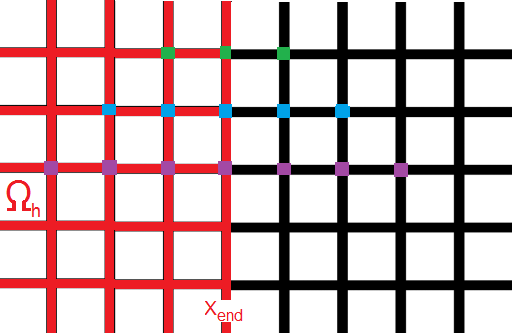
\includegraphics[width=2in]{Pictures/BoundaryPicture.png}
	\caption{Finite Differences near the computational boundary.}
	\label{fig:BoundaryFD}
  \end{center}
\end{figure}
two extra points and for $p=6$, it implies seven point stencil (purple color) with maximum three extra points outside the computational domain $\Omega_h$ (see Figure \ref{fig:BoundaryFD}). Same reasoning is implied for the $\partial^2 / \partial y^2$ derivative. The affected terms in equation \rf{Leq} which make use of the boundary function \rf{eqBCV} are the following:
\begin{equation*}
\frac{ \Delta_h u_h}{\beta}, \frac{ (E - \Delta_h)^{-1} ( (\beta -1)\Delta_h u_h) }{\beta}
\end{equation*}
The TS approach also requires time derivatives of both terms defined above
\begin{equation*}
\frac{ \Delta_h D^{(\tilde s)} (u_h)}{\beta}, \frac{ (E - \Delta_h)^{-1} ( (\beta -1)\Delta_h D^{(\tilde s)}(u_h) ) }{\beta}
\end{equation*}
for $\tilde s = 0, ..., s-2$.  Thus, $D^{\tilde s}(\widehat U_B(x , y, t))$  time derivative values outside the computational boundary $\partial \Omega_h$ are also used to extend the $p+1$ point stencil where needed (see Figure  \ref{fig:BoundaryFD}).


%The title of your section \href{mailto:#1}{{\mdseries\ttfamily #1}}}
\section{Introduction}

Papers should be written in English. Please use the JMPAG template
(the files \texttt{jmpag.sty} and \texttt{sample.tex}) to prepare
your tex file after the paper is accepted by the the JMPAG. You should put the files
\texttt{jmpag.sty} and \texttt{sample.tex} in the same folder to
work correctly. For detailed instructions in \LaTeX{} see, e.\,g.,
\URL{https://www.sharelatex.com/learn}. Please open both files \texttt{sample.tex} and
\texttt{sample.pdf} and read carefully all information in them
including details proceeded by \% sign (in the \TeX -file). In
particular, you should set the title of the paper, names of the
authors, their affiliations, addresses of affiliations, and
e-mail addresses just after \verb@\begin{document}@ and before
\verb@\BeginPaper@. After the command \verb@\BeginPaper@ you may
put your own macros if you need. Note that using  commands of the type \verb@\def@, the command \verb@\renewcommand@ and other  \verb@\renew@\ldots{}  are not allowed. Next, you should give the abstract
of the paper, keywords, and  the AMS Subject
Classification 2010 codes:
\URL{https://mathscinet.ams.org/msc/msc2010.html}. After that you
may begin the text of your paper. Please note that the footnotes
are not allowed throughout the paper. Place the list of
references at the end of the paper, using samples given in
\texttt{sample.tex}. The command \verb@\EndPaper@ is the last one
before \verb@\end{document}@. Note that you should run PDF\LaTeX{}
procedure of compilation for the pdf-file to show up correctly. Thus you obtain the pdf-file directly without dvi-file.
These are important instructions and explanations. Thank you for
your cooperation.





Please note that using cross-references is \textbf{mabdatory}. It
may require two \LaTeX{} compilations for the references to show
up correctly. Please use cross-references to all enumerated elements
(equations, sections, figures, theorems, etc.) in the
following way. The command  \verb@\label{name}@ should be used to
assign the identifier ``name'' to an element. The command
\verb@\ref{label-name}@ or \verb@\eqref{label-name}@  references the object you have marked before, see Subsections \ref{thrm}, \ref{list},
and \ref{fig}. The command  \verb@\bibitem{label-bibitem}@
should be used to
assign the identifier ``label-bibitem'' to a citation. The command
\verb@\cite{label-bibitem}@ or \verb@\cite[text]{label-bibitem}@ cites the item you have marked before, see Section \ref{citation}.


%The title of your subsection in the section
\subsection{A sample of theorem}\label{thrm}

\begin{theorem} \label{result1}
        Content of your theorem.
\end{theorem}

\begin{proof}
To refer to equations and statements in your paper, use the
commands \verb@\ref{label}@ and \verb@\eqref{label}@:
\eqref{Quotient}, \eqref{Multi}, \eqref{Equ3}, and Lemma \ref{L:
Lyapunov exponents}.
\end{proof}

\begin{theorem}[Main theorem] \label{result1a}
        Content of your theorem.
\end{theorem}

%The title of your subsection in the section
\subsection{A sample of lemma}

\begin{lemma} \label{L: Lyapunov exponents} State your lemma here.
\end{lemma}

\begin{proof}
Your proof statements.
\end{proof}

Text in definition and remark should not be slanted.

%The title of your subsection in the section
\subsection{A sample of remark}

\begin{remark}
Content of your remark.
\end{remark}

%The title of your subsection in the section
\subsection{A sample of definition}

\begin{definition} Sample: Let $\phi_{t}$ be an Anosmia flow on a
        compact space $V$ and $A \subset V$ a dense set. Say
        that the upper Lacunae exponents are
        \emph{$\frac{1}{2}$-pinched} on $A$ if


  \begin{equation}\label{Quotient}
        \sup_{x \in A} \frac{\max \{ |\bar{\lambda}|: \bar{\lambda} \
        \text{is a nonzero upper Lyapunov exponent at} \ x \}}
        {\min \{ |\bar{\lambda}|: \bar{\lambda} \ \text{is a
        nonzero upper Lyapunov exponent at} \ x\}}
         \leq 2.
  \end{equation}
\end{definition}

%The title of your  subsection in the section
\subsection{Examples of inserting figures}\label{fig}


 The JMPAG requires graphics to be sent in \texttt{jpeg}, \texttt{jpg}, \texttt{png},
or \texttt{pdf} format. Use the \texttt{graphicx} package  to
embed references to your graphics directly in a \LaTeX{} file. The
use of other packages are strictly prohibited. The \texttt{jpeg},
\texttt{jpg}, \texttt{png}, and \texttt{pdf} files will not be
physically included in the \LaTeX{} file. Each graphic must be
submitted as a separate file along with the \LaTeX{} document.
%The hard copies of the journal are printed in black and white.

Your may also create graphics using \texttt{TikZ} package. Please
do not use obsolete graphic packages (e.\,g., \texttt{picture},
\texttt{epic}, \texttt{eepic}, etc.) for creating your graphics.

Here are the examples of inserting  figures (see Figures
\ref{fig1}--\ref{fig:5}).

\begin{figure}[ht]
\begin{center}
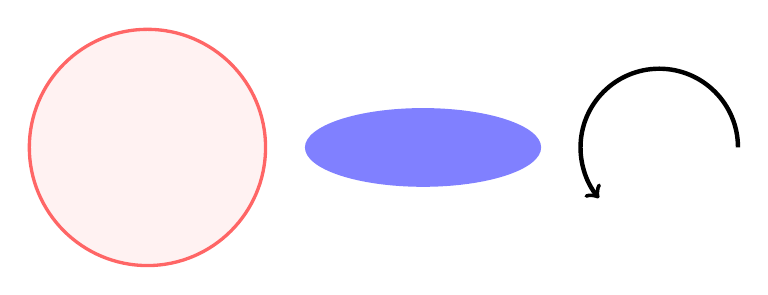
\begin{tikzpicture}% It requires \usepackage{tikz}
\filldraw[color=red!60, fill=red!5, very thick](-1,0) circle (1.5);
\fill[blue!50] (2.5,0) ellipse (1.5 and 0.5);
\draw[ultra thick, ->] (6.5,0) arc (0:220:1);
\end{tikzpicture}
  \caption{Here is the caption of your figure}\label{fig1}
  \end{center}
\end{figure}

\begin{figure}[ht]% It requires \usepackage{graphicx}
\begin{center}
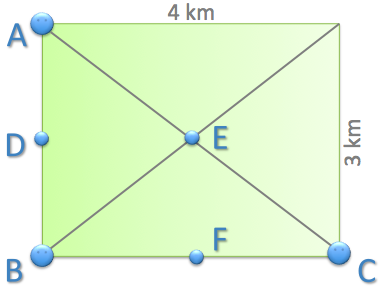
\includegraphics[width=2in]{pic1.png}
  \caption{Here is the caption of your figure}\label{AIMS}
  \end{center}
\end{figure}

\begin{figure}[ht]% It requires \usepackage{tikz,graphicx,subcaption}
\begin{center}
\begin{subfigure}[b]{0.45\linewidth}
\centering  \begin{tikzpicture}
\draw (0,0) -- (4,0);
\filldraw [gray] (2,0) circle (2pt);
\draw (0,-2) .. controls (2,0) .. (4,-2);
\draw (0,2) .. controls (1,0) and (3,0) .. (4,2);
\end{tikzpicture}
\centering \caption{\parbox[t]{0.6\textwidth}{Here is the caption of your figure 1}}
\label{fig:5.1}
\end{subfigure}
\begin{subfigure}[b]{0.45\linewidth}
\centering 
\includegraphics[width=2in]{tree.jpg}\\
\centering \caption{\parbox[t]{0.6\textwidth}{Here is the caption of your figure 2}}
\label{fig:5.2}
\end{subfigure}
      \caption{Here is the caption of your figures}\label{fig:5}
\end{center}
\end{figure}


%The title of your subsection  in the section
\subsection{Samples of enumerated lists}\label{list}

For creating enumerated lists, \textbf{only} the package
\texttt{enumitem} should be used. Please use the commands:
\verb@\arabic*@, \verb@\Roman*@, \verb@\roman*@, \verb@\Alph*@, or
\verb@\alph*@, with appropriate symbols of the point, parentheses,
or braces. Below we give some examples of enumerated lists.


Arabic numerals:
\begin{enumerate}[label=\upshape{\arabic*.},ref=\upshape{\arabic*}]
\item\label{la1}
Your first item.
\item\label{la2}
Your second item.
\item\label{la3}
Your third item.
\end{enumerate}
You may create labels and use the command \verb@\ref{label}@ to cite these items, e.\,g., \ref{la2}.

Roman numerals:
\begin{enumerate}[label=\upshape{(\roman*)},ref=\upshape{(\roman*)}]
\item\label{laa1}
your first item;
\item\label{laa2}
your second item;
\item\label{laa3}
your third item.
\end{enumerate}
You may create labels and use the command \verb@\ref{label}@ to cite these items, e.\,g., \ref{laa2}.

An alphabetical list:
\begin{enumerate}[label=\upshape{\Alph*)},ref=\upshape{\Alph*)}]
\item\label{laaa1}
your first item;
\item\label{laaa2}
your second item;
\item\label{laaa3}
your third item.
\end{enumerate}
You may create labels and use the command \verb@\ref{label}@ to cite these items, e.\,g., \ref{laaa2}.

A list with  sublists:
\begin{enumerate}[label=\upshape{\arabic*.},ref=\upshape{\arabic*}]
\item\label{lab1}
Your first item:
\begin{enumerate}[label=\upshape{\alph*)},ref=\upshape{\alph*)},topsep=1pt]
\item\label{laaab1}
your first subitem;
\item\label{laaab2}
your second subitem;
\item\label{laaab3}
your third subitem.
\end{enumerate}
\item\label{lab2}
Your second item.
\item\label{lab3}
Your third item:
\begin{enumerate}[label=\upshape{(\Roman*)},ref=\upshape{(\Roman*)},topsep=1pt]
\item\label{laab1}
your first subitem;
\item\label{laab2}
your second subitem;
\item\label{laab3}
your third subitem;
\item\label{laab4}
your forth subitem.
\end{enumerate}
\end{enumerate}
You may create labels and use the command \verb@\ref{label}@ to cite these items, e.\,g., \ref{lab1}\ref{laaab3}





%The title of your section
\section{How to align  math formulas}

To create your formulas, use the environments \texttt{gather},
\texttt{align}, \texttt{multline}, \texttt{aligned},
\texttt{split}, and others except the obsolete environment
\texttt{eqnarray}.

\begin{theorem} \label{result2}
        Content of your theorem.
\end{theorem}

In the proof below, we would like to show you how to align the math
formulas:
\begin{proof}[Proof of Theorem \ref{result2}]
Please refer to the following example and align your math formulas:
\begin{align}
    \eps{\theta} \wedge d\eps{\theta}^{n-1}& = (\theta_0 + \ep \alpha)
    \wedge (d(\theta_0 + \ep \alpha))^{n-1}
    \nonumber\\
    &= (\theta_0 + \ep \alpha) \wedge
    (d\theta_0)^{n-1} + \theta_0 \wedge d\theta_0^{n-1} - \ep d\left(\alpha \wedge
    \theta_0 \wedge d\theta_0^{n-2}\right)\nonumber\\
    &\qquad  + \theta_0 \wedge d\theta_0^{n-1} + \ep \alpha \wedge
    d\theta_0^{n-1}  \nonumber\\
    &= \theta_0 \wedge d\theta_0^{n-1} - \ep d\left(\alpha \wedge
    \theta_0 \wedge d\theta_0^{n-2}\right),\label{Multi}
\end{align}

It also can be aligned in the following way:

\begin{multline}
    \eps{\theta} \wedge d\eps{\theta}^{n-1} = (\theta_0 + \ep \alpha)
    \wedge (d(\theta_0 + \ep \alpha))^{n-1}
    \\
    = (\theta_0 + \ep \alpha) \wedge
    (d\theta_0)^{n-1} + \theta_0 \wedge d\theta_0^{n-1} - \ep d\left(\alpha \wedge
    \theta_0 \wedge d\theta_0^{n-2}\right)\\
      + \theta_0 \wedge d\theta_0^{n-1} + \ep \alpha \wedge
    d\theta_0^{n-1}  \\
    =\theta_0 \wedge d\theta_0^{n-1} - \ep d\left(\alpha \wedge
    \theta_0 \wedge d\theta_0^{n-2}\right),\label{Multi1}
\end{multline}



Here is other example if the math expression in [ ] exceeds one
line:

\begin{align}
 \int_0^T |u_0(t)|^2dt&  \leq \delta^{-1} \left[\int_0^T
(\beta(t)+\gamma(t))\, dt  \vphantom{\left(\int_0^T \right)^{\frac{2}{p}}}%to equalize brackets
\right.\nonumber\\
\label{Equ3}
&  \left.+T^{\frac{2(p-1)}{p}}\left(\int_0^T
|\dot{u}_0(t)|^p\,dt\right)^{\frac{2}{p}}
 +T^{\frac{2(p-1)}{p}}\left(\int_0^T |\dot{u}_0(t)|^p\,dt\right)^{\frac{2}{p}}\right].
\end{align}

 Please use the displaystyle if your formulas fully
occupy a paragraph, while use textstyle among the text.

For two equations:
\begin{align*}
A &= \theta_0 \wedge d\theta_0^{n-1} - \ep d\left(\alpha \wedge \theta_0 \wedge d\theta_0^{n-2}\right),\\
B&=\theta_1 \wedge d\theta_1^{n-1} - \ep d\left(\alpha \wedge \theta_1
\wedge d\theta_1^{n-2}\right).
\end{align*}
Please align your formulas nicely according to the above examples. Thanks.
\end{proof}


%The title of your section
\section{References}

A sample of the references you may find below. Please put your
references in alphabetical order. For abbreviations of names of
journals, use the list:
\URL{http://msc2010.org/MSC2010-CD/extras/serials.pdf}

%The title of your section
\section{Citations}\label{citation}

We use the package \texttt{cite} for creating citations. For citing
use the command \verb@\cite{label}@ or
\verb@\cite[text]{label}@, e.\,g., \cite{BFL},
\cite{Hoff,Whho,Serrin,BFL,BY,A22,quas,Mitt}, or \cite[Chapter
1]{rB}.

%%%%%%%%%%%%%%%%%%%%%%%%%%%%%%%%%%%%%%%%%%%%%%%%%%%%%%%%%%%%%%

%For acknowledgements section, please don't number the section, please begin it with \section*{Acknowledgements.}

\subsection*{Acknowledgments.} We would like to thank you for \textbf{following
the instructions above} very closely in advance. It will definitely
save us lot of time and expedite the process of your paper's
publication.

%%%%%%%%%%%%%%%%%%%%%%%%%%%%%%%%%%%%%%%%%%%%%%%%%%%%%%%%%%%%%%%%

\subsection*{Supports.} The first author is supported by the NSF grant xx-xxxx.

%%%%%%%%%%%%%%%%%%%%%%%%%%%%%%%%%%%%%%%%%%%%%%%%%%%%%%%%%%%%%%%

% References

\begin{thebibliography}{99}

% Example of multiple authors:
\bibitem{BFL}
Y. Benoist, P. Foulon and F. Labourie, % Use `and' connect the last two authors
\emph{Flots d'Anosov a distributions stable et instable differentiables,}
J. Amer. Math. Soc. \textbf{5} (1992), 33--74 (French).

%1
\bibitem{ChChr} C.I. Christov, 
\emph{An energy-consistent dispersive shallow-water model}, 
{\it Wave Motion}, \textbf{34} (2001), 161-174.

%2
\bibitem{EllipticProblem}
K. Angelow, N. Kolkovska, 
\emph{Numerical Study of Traveling Wave Solutions to 2D Boussinesq Equation},
Serdica J. Computing,  8, (2018) 3-4.

%3
\bibitem{BoundaryProblem}
K. Angelow, 
\emph{New Boundary Condition for the Two Dimensional Stationary Boussinesq Paradigm Equation},
International Journal of Applied Mathematics, (2018).

%4
\bibitem{FPS}
T. Lyche,
\emph{Fast Poisson Solvers and FFT}, 
Lecture Notes, University of Oslo, Norway

%5
\bibitem{chr-chr-07}
M.~Christou, C.~I.~Christov, Fourier–Galerkin method for 2D solitons of Boussinesq equation, 
Mathematics and Computers in Simulation, 74, (2007) 82 -- 92.
%6
\bibitem{chr-chr}
M.~Christou, C.~I.~Christov, Galerkin Spectral Method for the 2D Solitary
Waves of Boussinesq Paradigm Equation, CP 1186, (2009) 217 -- 225.
%7
\bibitem{Ch2012}
C.~I.~Christov,  Numerical implementation of the asymptotic boundary conditions
for steadily propagating 2D solitons of   Boussinesq type equation,       
Math. Computers  Simul., 82 (2012),  1079 -- 1092.
%8
\bibitem{Ch2011}
C.~I.~Christov, J. Choudhury, Perturbation solution  for the 2D Boussinesq equation,       
Mech. Res. Commun., 38 (2011),  274 -- 281.
%9
\bibitem{cher}
A.~Chertock, C.~Christov, A.~Kurganov, Central--upwind schemes for the  Boussinesq paradigm equation, Comp. Sci. High Performance Comp. IV, NNFM, 113, (2011), 267 -- 281.

\bibitem{dani}
C.~Christov, N.~Kolkovska, D.~Vasileva, On the numerical simulation of unsteady solutions for the 2D Boussinesq paradigm equation, LNCS, 6046  (2011), 386 -- 394.

\bibitem{chd-chr}
J.~Choudhury, C.~Christov, 2D  Solitary waves of  Boussinesq equation, CP75, (2005), 85 -- 90.
 
\bibitem{forn}
B.~Fornberg, 
\emph{Generation of Finite Difference Formulas on Arbitrarily Spaced Grids}, 
Math. Comput., 51(1988),  699 -- 706.

\bibitem{sam}
A.~Samarskii, The theory of difference schemes, M. Dekker,  2001.


\bibitem{A11}
FirstNameInitial.  MiddleNameInitial. LastName, % first name middle initial. and then last name.  Only the first character in the paper title is capitalized.
\emph{Title of the paper,}
Name of the Journal \textbf{Volume} (Year), StaringPage--EndingPage.



% Example of multiple authors:
\bibitem{BFL}
Y. Benoist, P. Foulon and F. Labourie, % Use `and' connect the last two authors
\emph{Flots d'Anosov a distributions stable et instable differentiables,}
J. Amer. Math. Soc. \textbf{5} (1992), 33--74 (French).

% Example of a paper translated in English:
\bibitem{BY}
M.Sh. Birman and D.R. Yafaev,
\emph{The spectral shift function,}  Algebra i Analiz \textbf{4} (1992), No. 5, 1--44 (Russian); Engl. transl.: St. Petersburg Math. J. \textbf{4} (1993), No. 5, 833--870.

% Example of a preprint  with 7 digits archive number:
\bibitem{quas}
M. Entov, L. Polterovich and F. Zapolsky,
\emph{Quasi-morphisms and the Poisson bracket,}
preprint, \arXiv{math/0605406}.

% Example of a thesis:
\bibitem{Hoff}
P. Hoffmann,
\emph{Torsion Cycles and Set Theoretic Complete Intersection},
Ph.D thesis, Washington University in St. Louis, 2006.

\bibitem{Mitt}
F. Mittelbach and M. Goossens, \emph{The LATEX Companion,} 2$^{nd}$ ed., Addison-Wesley Co., Reading,
MA, 2004.

% No author names:
\bibitem{Whho}
\emph{SARS Expert Committee, SARS in Hong Kong: From Experience to
Action}, Report of Hong Kong SARS Expert Committee,
2003. Available from: \URL{http://www.sars-expertcom.gov.hk/english/reports/reports.html}.


% Example of a paper in Academic Press or a book:
\bibitem{Serrin}
J. Serrin,
\emph{Gradient estimates for solutions of nonlinear elliptic and parabolic equations,}
Contributions to Nonlinear Functional Analysis (eds. E.H. Zarantonello and Author 2), Academic Press, 1971, 33--75.

% Example of a book in the reference:
\bibitem{rB}
J.  Smoller,
\emph{Shock Waves and Reaction-Diffusion Equations},
2$^{nd}$ ed.,  Springer-Verlag, New York, 1994.

% Example of a preprint  with 8 digits archive number:
\bibitem{Te2008}
A. Teplinsky,
\emph{Herman's theory revisited,} preprint,
\arXiv{0707.0078}.

%
\bibitem{A22}
C.  Wolf,
\emph{A mathematical model for the propagation of a hantavirus in structured populations,}
Discrete Contin. Dyn. Syst. Ser. B \textbf{4} (2004), 1065--1089.



\end{thebibliography}


%%%%%%%%%%%%%%%%%%%%%%%%%%%%%%

\EndPaper%%%%  do not remove this command

%%%%%%%%%%%%%%%%%%%%%%%%%%%%%%%%%%%%%%%%%%%%%%%%%%%%%%%

\end{document}
